\documentclass[../main]{subfiles}
\begin{document}
\chapter{Ecuaciones de Estado}
Las ecuaciones de estado modelan el comportamiento de una sustancia y se pueden representar de la siguiente manera:
\begin{equation}
    f(p,V,T)=0
\end{equation}
donde:
\begin{itemize}
    \item $p$ es la presión.
    \item $V$ es el volumen.
    \item $T$ es la temperatura.
\end{itemize}
\section{Ecuación de estado térmica}
Partiendo de la ley de gas ideal:
\begin{equation}
    p=\dfrac{n RT}{V}
\end{equation}
la cual podemos expresar de la siguiente forma:
\begin{equation}
    pV=nRT
\end{equation}
la cual es conocida como \textbf{ecuación de Clapeyron-Mendeleiev}. Donde:
\begin{equation}
    n=\dfrac{m}{M}=\dfrac{\text{masa de la sustancia}}{\text{masa molar}}
\end{equation}
\section{Ecuación de estado calórica}
La ecuación de estado calórica se expresa de la siguiente forma:
\begin{equation}
    U=U_0+C_v(T-T_0)
\end{equation}
esta ecuación se demostrará mas adelante.

\begin{itemize}
    \item $U$ es la energía interna.
    \item $C_v$ es la capacidad calorífica a $V=cte$.
\end{itemize}

\section*{Procesos Termodinámicos}

\begin{itemize}
    \item Isotérmico ($T=cte$).
    \item Isobárico ($p=cte$).
    \item Isocórico ($V=cte$).
    \item Politrópico ($C=cte$).
    \item Adiabático $\left(C=\dfrac{\delta Q}{dT}=0\right)$.
\end{itemize}

\section{Proceso Isotérmico (T=cte)}

\begin{minipage}{0.49\textwidth}
    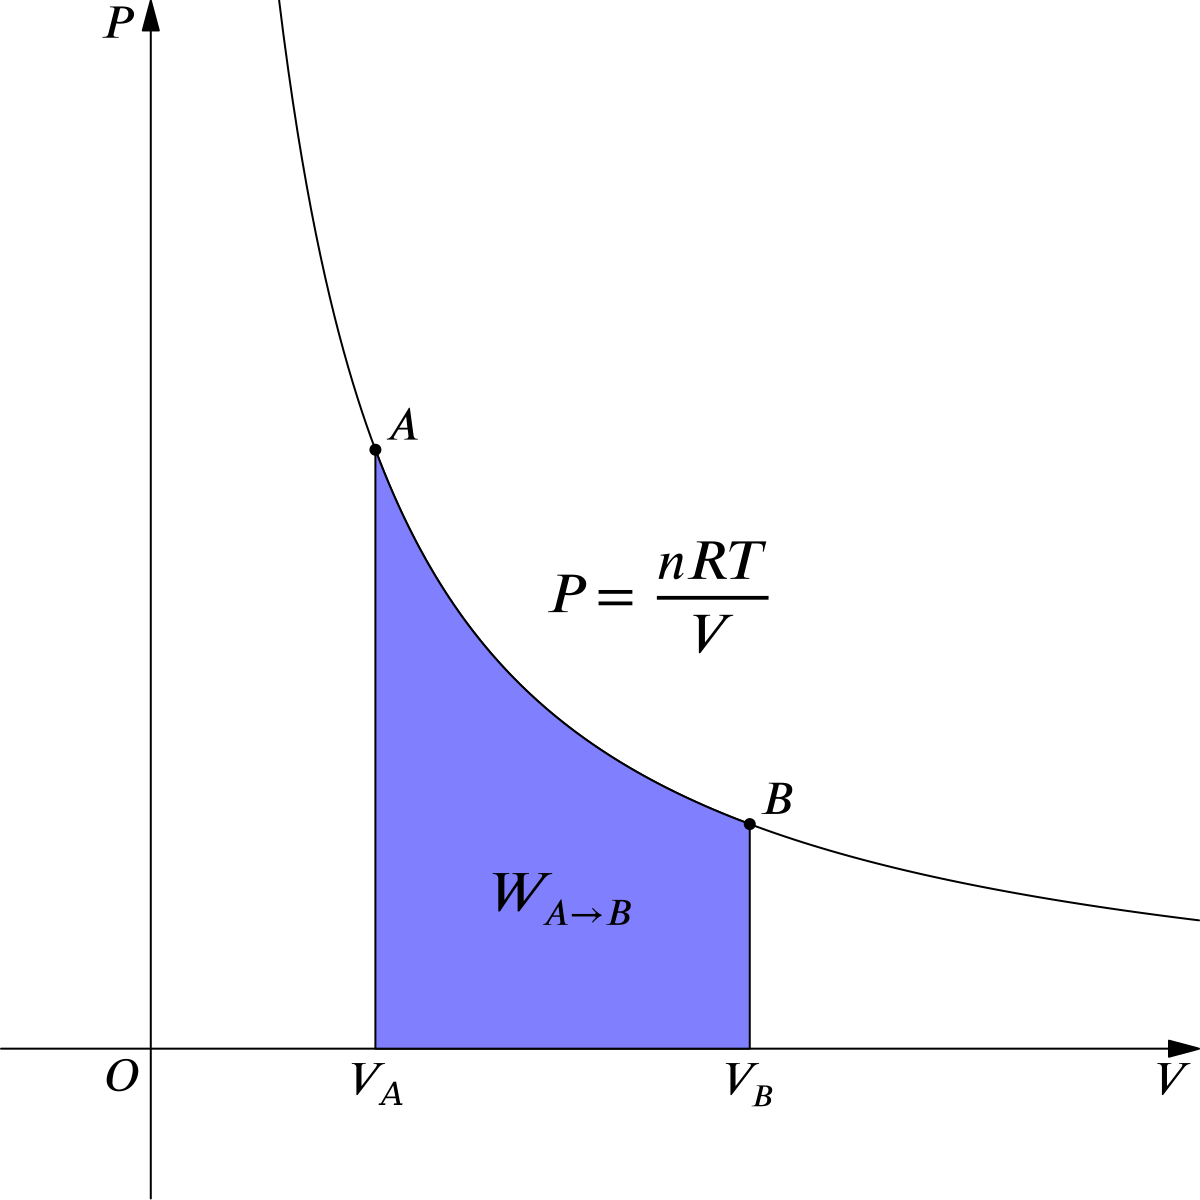
\includegraphics[width=\linewidth]{../images/isotermico.png}
\end{minipage}
\begin{minipage}{0.49\textwidth}
    Considerando la ec. de Clapeyron-Mendeleiev y que $T=cte$, tenemos que $nRT=c_1$.
    \begin{equation*}
        pV=nRT=c_1
    \end{equation*}
    De modo que:
    \begin{equation}
        pV=c_1 \rightarrow p=\dfrac{c_1}{V}=p(V)
    \end{equation}
    donde $c_1=nRT$.
\end{minipage}

\section{Proceso Isobárico (p=cte)}

\begin{minipage}{0.49\textwidth}
    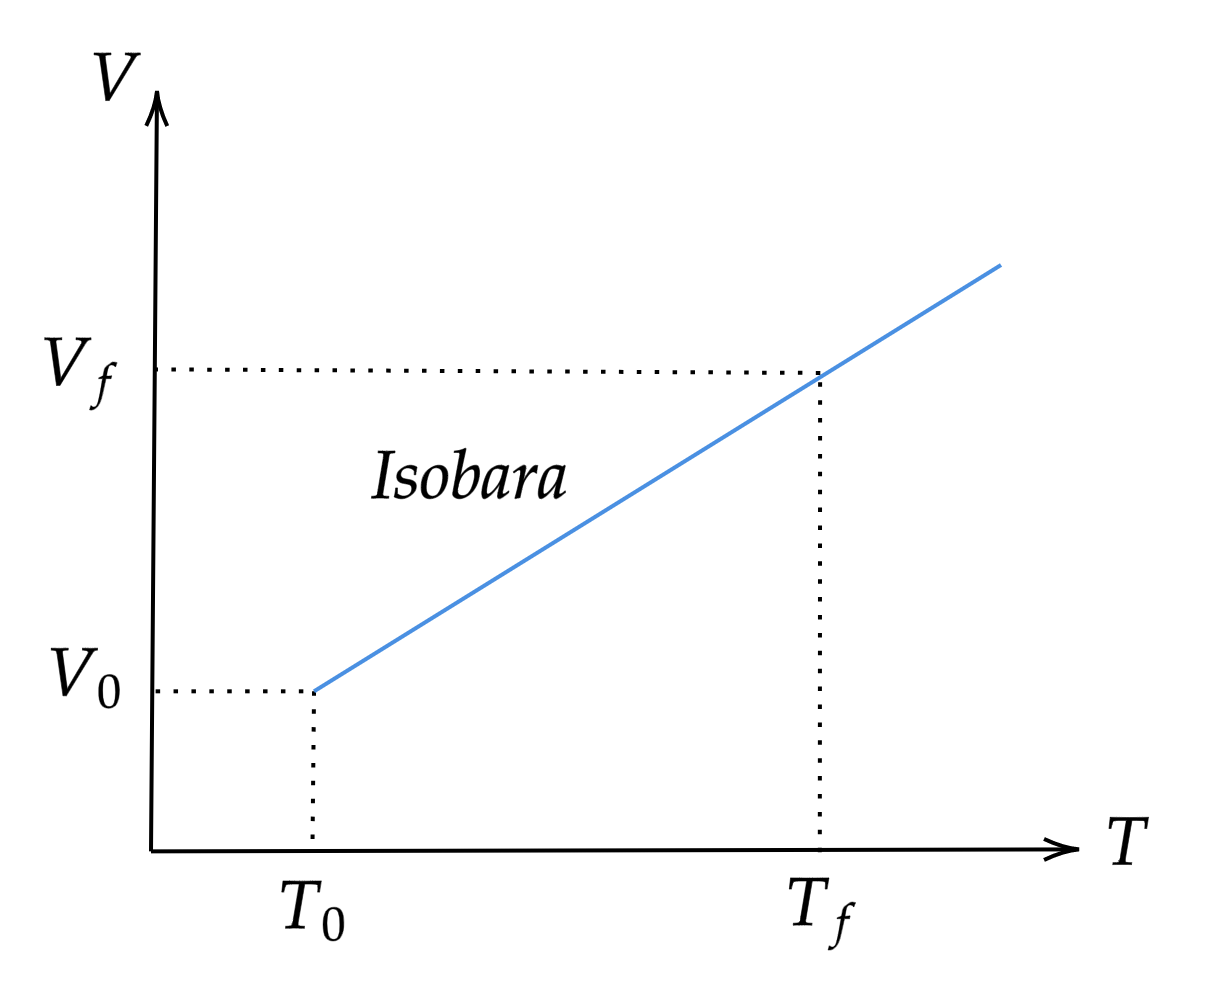
\includegraphics[width=\linewidth]{../images/isobara.png}
\end{minipage}
\begin{minipage}{0.49\textwidth}
    Partiendo de la ec. de Clapeyron-Mendeleiev, como $p=cte$ entonces:
    \begin{equation*}
        pV=nRT \rightarrow V=\dfrac{nRT}{p}
    \end{equation*}
    donde $\dfrac{nR}{p}=cte=c_2$, entonces:
    \begin{equation*}
        V=\dfrac{nRT}{p}=c_2 T=V=f(T)
    \end{equation*}
\end{minipage}

\section{Proceso Isocórico}
\begin{minipage}{0.49\textwidth}
    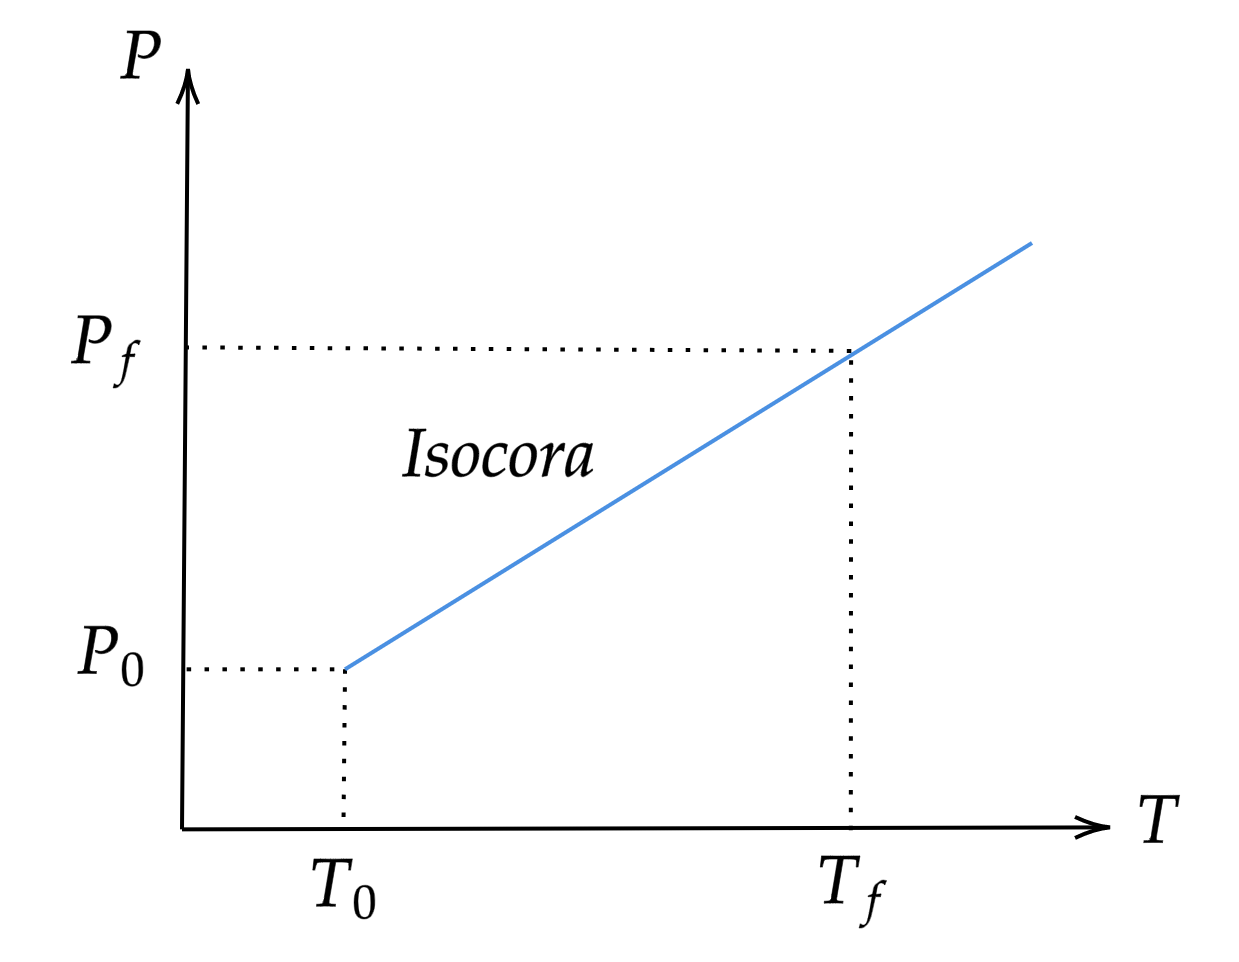
\includegraphics[width=\linewidth]{../images/isocora.png}
\end{minipage}
\begin{minipage}{0.49\textwidth}
    Partiendo de la ec. de Clapeyron-Mendeleiev, como $V=cte$ entonces:
    \begin{equation*}
        pV=nRT \rightarrow p=\dfrac{nRT}{V}
    \end{equation*}
    donde $\dfrac{nR}{V}=cte=c_3$, entonces:
    \begin{equation*}
        p=\dfrac{nRT}{V}=c_3 T=f(T)
    \end{equation*}
\end{minipage}
\chapter{Energía interna}
Vamos a definir la función  de estado llamada energía interna la cual va a depender de la temperatura y el volumen(para un sistema cerrado):
\begin{equation}
    U=U(T,V)
\end{equation}
Para un sistema abierto la energía interna dependerá también de $N$ la cual significa el número de componentes del sistema:
\begin{equation}
    U=U(T,V,N)
\end{equation}
Calculamos la evolución energetica del sistema hallando la diferencial de $U$:
\begin{align}
    dU & =\left( \pdv{U}{T} \right)_V dT + \left( \pdv{U}{V} \right)_T dV \\
    dU & =\alpha(T)dT+\beta(V)dV
\end{align}
\textbf{Observación:}
\begin{equation}
    \boxed{\int dU=\int_{T_0}^T \alpha(T)dT+\int_{V_0}^V \beta(V)dV}
\end{equation}

\section{Trabajo calorífico elemental}
Tenemos que el trabajo calorifico puede ser expresado como:
\begin{align}
    \delta W & =\sum_{i=1}^{\ell} A_i d a_i          \\
    \delta W & =A_1 da_1+\cdots + A_{\ell} da_{\ell}
\end{align}
donde:
\begin{itemize}
    \item $a_i$ es la i-ésima coordenada generalizada.
    \item $A_u$ es la i-ésima fuerza generalizada.
    \item $\ell$ son los grados de libertad
\end{itemize}
\begin{minipage}{0.49\textwidth}
    Otra forma de expresarlo es:
    \begin{equation}
        \delta W=\mathbf{F} \cdot d \mathbf{r}=pdV
    \end{equation}
    Expresado en su forma integral:
    \begin{equation}
        W=\int \delta W=\int_{V_0}^{V}p dV
    \end{equation}
\end{minipage}
\begin{minipage}{0.49\textwidth}
    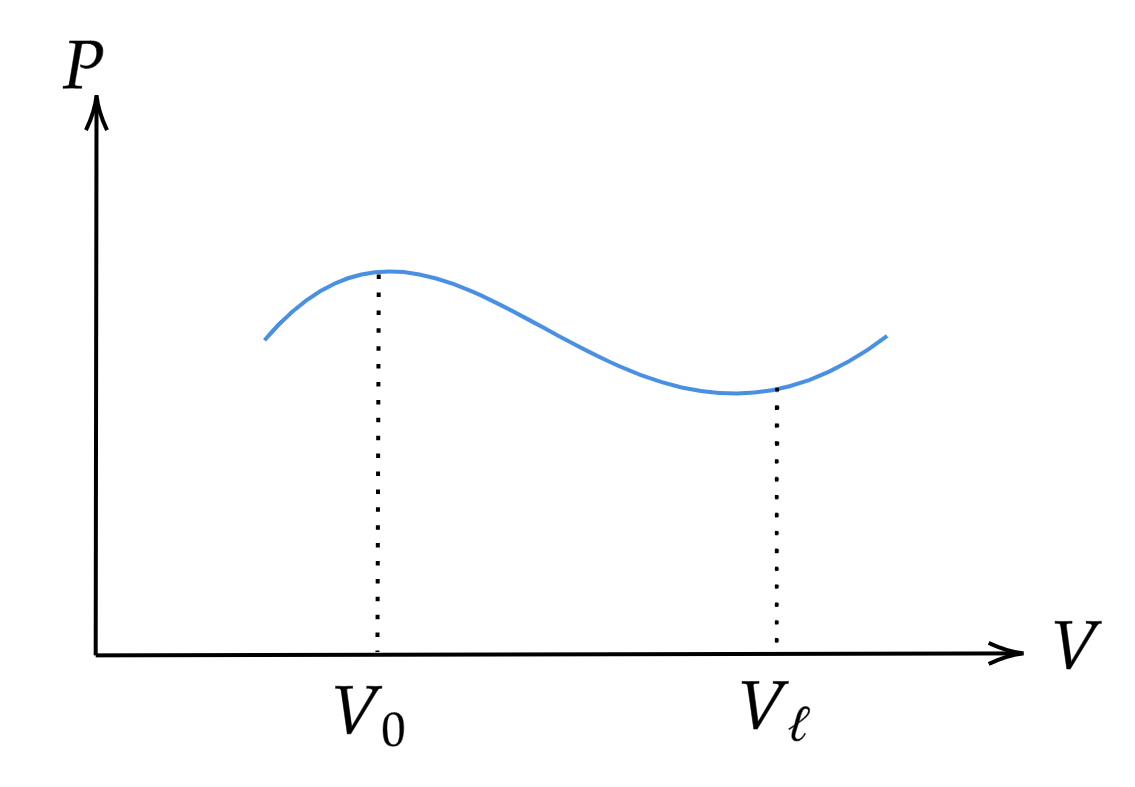
\includegraphics[scale=0.23]{../images/diagram-20230116.png}
\end{minipage}

\chapter{Primera ley de la termodinámica}
Conservación de la energía calorífica:
\begin{align}
    Q=U_2-U_1+W \\
    \delta Q=dU+\delta W
\end{align}
Si $\delta W = p dV$, entonces:
\begin{equation}
    \delta Q=dU+pdV
\end{equation}
la cual es la forma diferencial de la Primera ley de la termodinámica.
\begin{equation}
    \delta Q=\left( \pdv{U}{T}\right)_V dT + \left[ \left(\pdv{U}{V}\right)_T+p\right]dV
\end{equation}
donde por la \textbf{Ley de Joule} se cumple para el gas ideal que:
\begin{equation}
    \left(\pdv{U}{V}\right)_T=0
\end{equation}
\section{Funciones termodinámicas}
\textbf{Función de proceso:} Dependen solo del camino recorrido. (Trabajo, calor,etc)
\begin{equation}
    V_{1\rightarrow 2}=\int_{1\rightarrow 2} dV
\end{equation}
\textbf{Función de estado:} Dependen del estado inicial y final. (Entropia, Entalpia,etc)
\begin{equation}
    \int_{(1-2)}d\mu =\int_1^2 d\mu=\mu_2-\mu_1=\mu_{(2)}-\mu_{(1)}
\end{equation}

\section{Aplicación de la primera ley de la Termodinámica}

Primera definición de las capacidades caloríficas:

\begin{equation}
    C=\dfrac{\delta Q}{dT}
\end{equation}
Si $V=cte$:
\begin{equation}
    C_v=[C]_v
\end{equation}
Si $p=cte$:
\begin{equation}
    C_p=[C]_p
\end{equation}
\begin{enumerate}
    \item Para $C=C_v$, donde el volumen es constante y $dV=0$: \\
          Si $U=U(T,V)$:
          \begin{align}
              \delta Q & =\left(\pdv{U}{T}\right)_V dT+\left( \pdv{U}{V}\right)_T dV+pdV           \\
              \delta Q & =\left(\pdv{U}{T}\right)_V dT+\left[\left( \pdv{U}{V}\right)_T+p\right]dV
              \label{ec30}
          \end{align}
          Si $C=C_v$, donde el volumen es constante. Sabemos que la capacidad calorífica esta definida de forma general como:
          \begin{equation}
              C=\dfrac{dQ}{dT}
              \label{ec31}
          \end{equation}
          Y para el volumen constante reemplazamos \eqref{ec30} en \eqref{ec31}:
          \begin{align}
              C_v & =\left[\dfrac{\displaystyle \left(\pdv{U}{T}\right)_V dT+\left[\left( \pdv{U}{V}\right)_T+p\right]dV}{dT}\right]_V  \\
              C_v & = \left(\pdv{U}{T}\right)_V \dfrac{dT}{dT}+\left[ \left(\pdv{U}{V}\right)_T+p\right]\underbrace{\dfrac{dV}{dT}}_{0} \\
              C_v & =\left(\pdv{U}{T}\right)_V \dfrac{dT}{dT}=\left(\pdv{U}{T}\right)_V
          \end{align}
    \item Calcular $U$ si se tiene $C_v$ donde $dV=0$:
          Si obtenemos la derivada total de la energía interna donde $U=U(T,V)$, obtenemos:
          \begin{equation}
              dU=\left( \pdv{U}{T} \right)_V dT+\left( \pdv{U}{V} \right)_T dV
          \end{equation}
          Como el volumen es constante, entonces $dV=0$, quedándonos así:
          \begin{equation}
              dU=\left( \pdv{U}{T} \right)_V dT
          \end{equation}
          Pero sabemos que la capacidad calorífica a volumen constante esta definida como:
          \begin{equation}
              C_v=\left( \pdv{U}{T} \right)_V dT
          \end{equation}
          Reemplazamos e integramos:
          \begin{align*}
              dU                & =C_v dT                  \\
              \int_{U_0}^{U} dU & =\int_{T_0}^T C_v dT     \\
              U-U_0             & =\int_{T_0}^T C_v dT     \\
              U                 & =U_0+\int_{T_0}^T C_v dT
          \end{align*}
    \item Calcular $C=C_p$ donde la presión es constante y $dp=0$:\\
          Si $U=U(T,V)$:
          \begin{align}
              \delta Q & =\left(\pdv{U}{T}\right)_V dT+\left( \pdv{U}{V}\right)_T dV+pdV           \\
              \delta Q & =\left(\pdv{U}{T}\right)_V dT+\left[\left( \pdv{U}{V}\right)_T+p\right]dV
              \label{ec36}
          \end{align}
          Si $C_p$ esta definido como:
          \begin{equation}
              C_p=\left[ \dfrac{\delta Q}{dT}\right]_p
              \label{ec37}
          \end{equation}
          Reemplazamos \eqref{ec36} en \eqref{ec37}:
          \begin{align}
              C_p & =\left[ \dfrac{ \displaystyle \left(\pdv{U}{T}\right)_V dT+\left[\left( \pdv{U}{V}\right)_T+p\right]dV}{dT}\right]_p \\
              C_p & =\left[ \left(\pdv{U}{T}\right)_V+\left[\left(\pdv{U}{V}\right)_T+p\right]\dfrac{dV}{dT}\right]_p
          \end{align}
          Si $\displaystyle C_v=\left( \pdv{U}{T}\right)_V$:
          \begin{align}
              C_p & =C_v\left[ \left[\left(\pdv{U}{V}\right)_T+p\right]\dfrac{dV}{dT}\right]_p
              \label{ec40}
          \end{align}
          Si consideramos al volumen como una función que depende de $T$ y $p$:
          \begin{equation}
              V=V(T,p)
          \end{equation}
          hallamos su diferencial total:
          \begin{align}
              dV=\left(\pdv{V}{T}\right)_p+\left(\pdv{V}{p}\right)_T dp
          \end{align}
          en el caso cuando la presión es constante queda:
          \begin{equation}
              dV=\left( \pdv{V}{T}\right)_p
              \label{ec43}
          \end{equation}
          Reemplazamos \eqref{ec40} en \eqref{ec43}:
          \begin{equation}
              C_p=C_v+\left[ \left[\left(\pdv{U}{V}\right)_T+p\right]\dfrac{\partial V}{dT}\right]_p
          \end{equation}
\end{enumerate}
\section{Primera ley para un sistema abierto}
Para un sistema abierto monocomponente la primera ley se expresa como:
\begin{equation}
    \delta Q=dU+pdV-d \varepsilon
\end{equation}
donde $d \varepsilon= \mu dN$(sistema monocomponente)\footnote{$\mu$ es conocido como el potencial quimico.}, $d \varepsilon \approx dN$. \\
De forma general tenemos:
\begin{equation}
    \delta Q = dU+pdV-\sum_{i=1}^n \mu_i dN_i
\end{equation}
\chapter{Segunda ley de la termodinámica}
\section{Entropía}
Conocemos una nueva función de estado llamada entropía denotada por $S$ la cual es la encargada de caracterizar el nivel de organización de las componentes del sistema(orden o desorden).
\begin{align}
    \underbrace{dS}_{efecto}\sim \underbrace{\delta Q}_{causa} \\
    \delta Q= \lambda dS
\end{align}
donde $\lambda=\lambda(\underbrace{a_1,a_2, \cdots, a_n}_{par\acute{a}metros}, T)$ y $\lambda$ es conocido también como \textit{multiplicador de Lagrange}.
\begin{equation}
    \lambda = \lambda(a_1,a_2,\cdots, a_n,T)=\lambda(T)
\end{equation}
de modo que tenemos de forma diferencial:

\begin{equation}
    \delta Q=TdS
\end{equation}

\begin{minipage}{0.49\textwidth}
    O también:
    \begin{equation}
        dS= \dfrac{\delta Q}{T}
    \end{equation}
    Si integramos:
    \begin{align}
        \int_{(1)}^{(1)}dS & =\oint \dfrac{\delta Q}{T}  \\
        0                  & = \oint \dfrac{\delta Q}{T}
    \end{align}
    Esta integral se conoce como \textit{Integral de Clausius}.
\end{minipage}
\begin{minipage}{0.49\textwidth}
    \begin{center}
        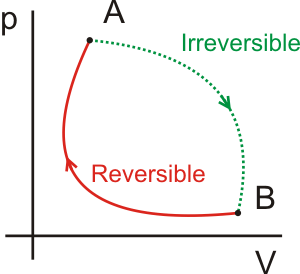
\includegraphics[scale=0.6]{../images/ciclo_irrev.png}
    \end{center}
\end{minipage}
\chapter{Ecuación Fundamental de la termodinámica}
Teniendo la primera ley de la termodinamica:
\begin{equation}
    \delta Q=dU+pdV
\end{equation}
y la segunda ley de la termodinamica:
\begin{equation}
    \delta Q=TdS
\end{equation}
Podemos unificar ambas en una sola ecuación:
\begin{equation}
    TdS=dU+pdV
\end{equation}
la cual llamaremos como \textbf{Ecuación fundamental de la Termodinámica}(EFT).
\section{Expresión analítica para entropía con gas ideal}
Recordando la ecuación de Clapeyron Mendeleiev:
\begin{equation}
    PV=nRT
\end{equation}
Si:
\begin{equation}
    dS= \dfrac{\delta Q}{T}=\dfrac{dU+pdV}{T}
    \label{ec58}
\end{equation}
Si despejamos $p$ de la ecuación de Clapeyron Mendeleiev:
\begin{equation}
    p=\dfrac{nRT}{V}
    \label{ec59}
\end{equation}
Hallamos el diferencial de la energia interna definida como $U=U(T,V)$:
\begin{align}
    dU & =\left( \pdv{U}{T}\right)_V dT+\underbrace{\left( \pdv{U}{V}\right)_T}_{ley \ de \ joule} dV \\
    dU & =C_v dT+(0)dV                                                                                \\
    dU & =C_v dT
    \label{ec62}
\end{align}
Reemplazando en \eqref{ec58}:
\begin{align}
    dS & =\dfrac{dU+pdV}{T}                \\
    dS & =\dfrac{Cv dT+pdV}{T}             \\
    dS & =C_v \dfrac{dT}{T}+\dfrac{p}{T}dV
\end{align}
Reemplazando la ecuación \eqref{ec59} e integrando nos queda:
\begin{align}
    dS               & =C_v \dfrac{dT}{T}+nR \dfrac{dV}{V}                                           \\
    \int_{S_0}^{S}dS & =\int_{T_0}^{T}C_v \dfrac{dT}{T}+\int_{V_0}^V nR \dfrac{dV}{V}                \\
    S-S_0            & =C_v \ln{\left(\dfrac{T}{T_0}\right)}+nR \ln{\left(\dfrac{V}{V_0}\right)}     \\
    S                & =S_0+C_v \ln{\left(\dfrac{T}{T_0}\right)}+nR \ln{\left(\dfrac{V}{V_0}\right)}
\end{align}
\section{Energía interna para un sistema cerrado}
De la ecuación fundamental de la termodinámica:
\begin{equation}
    TdS=dU+pdV
\end{equation}
Despejamos $U$:
\begin{equation}
    dU=TdS-pdV
    \label{ec71}
\end{equation}
Si $U=U(S,V)$, hallamos su diferencial total:
\begin{equation}
    dU=\left( \pdv{U}{S}\right)_V dS+\left( \pdv{U}{V}\right)_S dV
    \label{ec72}
\end{equation}
Igualamos tanto la ecuación \eqref{ec71} y la ecuación \eqref{ec72}:
\begin{equation}
    TdS-pdV=\left( \pdv{U}{S}\right)_V dS+\left( \pdv{U}{V}\right)_S dV
\end{equation}
Si comparamos términos notamos que:
\begin{equation}
    \left\{
    \begin{array}{l}
        T=\left(\displaystyle \pdv{U}{S}\right)_V \\ \\
        p=-\left(\displaystyle \pdv{U}{V}\right)_S
    \end{array}
    \right.
\end{equation}
\section{Energía libre de Helmholtz para un sistema cerrado}
Si tenemos una función $F$ denominada energía libre de Helmholtz la cual depende de la temperatura y el volumen:
\begin{equation}
    F=F(T,V)
\end{equation}
Hallamos la diferencial total para conocer la evolución energética del sistema:
\begin{equation}
    dF=\left( \pdv{F}{T}\right)_V dT+\left( \pdv{F}{V} \right)_T dV
    \label{ec76}
\end{equation}
de la EFT:
\begin{equation}
    TdS=dU+pdV
    \label{ec77}
\end{equation}
Aplicando una herramienta matematica:
\begin{align}
    d[ST] & =SdT+TdS   \\
    TdS   & =d[ST]-SdT
\end{align}
Reemplazando en \eqref{ec77}:
\begin{align}
    d[ST]-SdT & =dU+pdV   \\
    d[U-TS]   & =-SdT-pdV
\end{align}
donde $U-TS=F$, de modo que:
\begin{equation}
    dF=-SdT-pdV
    \label{ec82}
\end{equation}
Igualamos las ecuaciones \eqref{ec76} y \eqref{ec82}:
\begin{align}
    \left( \pdv{F}{T}\right)_V dT+\left( \pdv{F}{V} \right)_T dV=-SdT-pdV
\end{align}
Comparando términos obtenemos que:
\begin{equation}
    \left\{
    \begin{array}{l}
        S=-\left(\displaystyle \pdv{F}{T}\right)_V \\ \\
        p=-\left(\displaystyle \pdv{F}{V}\right)_T
    \end{array}
    \right.
\end{equation}

\section{Entalpía para un sistema cerrado}
Definimos una función energética $H$ denominada entalpía que depende de las variables $S$ y $p$:
\begin{equation}
    H=H(S,p)
\end{equation}
Hallamos la evolución energética del sistema:
\begin{equation}
    dH=\left( \pdv{H}{S}\right)_p dS+\left( \pdv{H}{p}\right)_S dP
    \label{ec86}
\end{equation}
Recordamos la EFT:
\begin{equation}
    TdS=dU+pdV
    \label{ec87}
\end{equation}
Se puede comprobar que:
\begin{equation}
    pdV=d[pV]-Vdp
    \label{ec88}
\end{equation}
Si reemplazamos \eqref{ec88} en \eqref{ec87}:
\begin{align}
    TdS     & =dU+d[pV]-Vdp \\
    TdS+Vdp & =d[U+pV]      \\
    d[U+pV] & =TdS+Vdp
\end{align}
donde $H=U+pV$, de modo que:
\begin{equation}
    dH=TdS+Vdp
    \label{ec92}
\end{equation}
Comparamos las ecuaciones \eqref{ec92} y \eqref{ec86}:
\begin{equation}
    \left( \pdv{H}{S}\right)_p dS+\left( \pdv{H}{p}\right)_S dP=TdS+Vdp
\end{equation}
De modo que:
\begin{equation}
    \left\{
    \begin{array}{l}
        T=\displaystyle \left( \pdv{H}{S} \right)_{p} \\ \\
        V=\displaystyle \left(\pdv{H}{p}\right)_{S}
    \end{array}
    \right.
\end{equation}

\section{Energía de Gibbs para un sistema cerrado}
Definimos una función energética $G$ denominada energía de Gibbs la cual depende de las variables $p$ y $T$:
\begin{equation}
    G=G(p,T)
\end{equation}
Hallamos la evolución energética del sistema:
\begin{equation}
    dG=\left( \pdv{G}{p}\right)_T dp+\left( \pdv{G}{T}\right)_p dT
    \label{ec96}
\end{equation}
La EFT:
\begin{equation}
    TdS=dU+pdV
    \label{ec97}
\end{equation}
Si:
\begin{align}
    TdS & =d[TS]-SdT \\
    pdV & =d[PV]-Vdp
\end{align}
Reemplazando en \eqref{ec97}:
\begin{align}
    d[TS]-SdT  & =dU+d[PV]-Vdp \\
    Vdp-SdT    & =d[U+pV-TS]   \\
    d[U+pV-TS] & = Vdp-Sdt
\end{align}
donde $G=U+pV-TS$, de modo que:
\begin{equation}
    dG=Vdp-Sdt
    \label{ec103}
\end{equation}
Comparamos \eqref{ec96} y \eqref{ec103}:
\begin{equation}
    \left( \pdv{G}{p}\right)_T dp+\left( \pdv{G}{T}\right)_p dT=Vdp-Sdt
\end{equation}
De modo que:
\begin{equation}
    \left\{
    \begin{array}{l}
        V=\displaystyle \left( \pdv{G}{p} \right)_{T} \\ \\
        S=-\displaystyle \left(\pdv{G}{T}\right)_{p}
    \end{array}
    \right.
\end{equation}

\chapter{Segunda Ley de la termodinámica para un sistema abierto monocomponente}
Recordando la primera ley:
\begin{equation}
    \delta Q = dU+pdV-\mu dN
\end{equation}
Recordando la segunda ley:
\begin{equation}
    \delta Q = TdS
\end{equation}
Si igualamos ambas leyes, obtenemos la ecuación fundamental de la Termodinamica(EFT):
\begin{equation}
    TdS=dU+pdV-\mu dN
\end{equation}
\section{Energía interna para un sistema abierto monocomponente}
Despejamos $U$ de la EFT:
\begin{equation}
    dU=TdS-pdV+\mu dN
\end{equation}
donde $U=U(S,V,N)$, lo diferenciamos:
\begin{equation}
    dU=\left( \pdv{U}{S} \right)_{V,N}dS+\left(\pdv{U}{V}\right)_{S,N}dV+\left( \pdv{U}{N}\right)_{S,V}dN
\end{equation}
Comparamos ambas ecuaciones y obtenemos:
\begin{equation}
    TdS-pdV+\mu dN=\left( \pdv{U}{S} \right)_{V,N}dS+\left(\pdv{U}{V}\right)_{S,N}dV+\left( \pdv{U}{N}\right)_{S,V}dN
\end{equation}
de modo que:
\begin{equation}
    \left\{
    \begin{array}{l}
        T=\displaystyle \left( \pdv{U}{S} \right)_{V,N} \\ \\
        p=-\displaystyle \left(\pdv{U}{V}\right)_{S,N}  \\ \\
        \mu=\displaystyle \left( \pdv{U}{N}\right)_{S,V}
    \end{array}
    \right.
\end{equation}
\section{Energía libre de Helmholtz para un sistema abierto monocomponente}
Si tenemos el potencial de Helmholtz definido por:
\begin{equation}
    F=F(T,V,N)
\end{equation}
Utilizando la EFT:
\begin{equation}
    TdS=dU+pdV-\mu dN
\end{equation}
Si:
\begin{equation*}
    TdS=d(TS)-SdT
\end{equation*}
Reemplazamos y obtenemos:
\begin{align}
    dU      & =d(TS)-SdT-pdV+\mu dN \\
    d(U-TS) & =-SdT-pdV+\mu dN
\end{align}
De modo que $F=U-TS$, si diferenciamos $F$, obtenemos:
\begin{equation}
    dF=\left( \pdv{F}{T}\right)_{V,N}dT+\left( \pdv{F}{V} \right)_{T,N}dV+\left( \pdv{F}{N}\right)_{T,V}dN
\end{equation}
De modo que si comparamos ambas ecuaciones:
\begin{equation}
    \left( \pdv{F}{T}\right)_{V,N}dT+\left( \pdv{F}{V} \right)_{T,N}dV+\left( \pdv{F}{N}\right)_{T,V}dN=-SdT-pdV+\mu dN
\end{equation}
\begin{equation}
    \left\{
    \begin{array}{l}
        S=\displaystyle -\left( \pdv{F}{T}\right)_{V,N}  \\ \\
        p=\displaystyle -\left( \pdv{F}{V} \right)_{T,N} \\ \\
        \mu=\displaystyle \left( \pdv{F}{N}\right)_{T,V}
    \end{array}
    \right.
\end{equation}
\section{Entalpia para un sistema abierto monocomponente}
Si tenemos la entalpia definida por:
\begin{equation}
    H=H(S,p,N)
\end{equation}
Utilizando la EFT:
\begin{equation}
    TdS=dU+pdV-\mu dN
\end{equation}
Si:
\begin{equation}
    pdV=d(pV)-Vdp
\end{equation}
Reemplazamos y obtenemos:
\begin{align}
    dU      & =TdS-d(pV)+Vdp+\mu dN \\
    d(U+pV) & =TdS+Vdp+\mu dN
\end{align}
De modo que $H=U+pV$, si diferenciamos $H$, obtenemos:
\begin{equation}
    dH=\left( \pdv{H}{S} \right)_{p,N}dS+\left( \pdv{H}{p}\right)_{S,N}dp+\left ( \pdv{H}{N} \right)_{S,p}dN
\end{equation}
Comparamos ambas ecuaciones:
\begin{equation}
    \left( \pdv{H}{S} \right)_{p,N}dS+\left( \pdv{H}{p}\right)_{S,N}dp+\left ( \pdv{H}{N} \right)_{S,p}dN=TdS+Vdp+\mu dN
\end{equation}
\begin{equation}
    \left\{
    \begin{array}{l}
        T=\displaystyle \left( \pdv{H}{S} \right)_{p,N} \\ \\
        V=\displaystyle \left( \pdv{H}{p}\right)_{S,N}  \\ \\
        \mu=\displaystyle \left ( \pdv{H}{N} \right)_{S,p}
    \end{array}
    \right.
\end{equation}
\section{Energia de Gibbs para un sistema abierto monocomponente}
Si tenemos el potencial de Gibbs definido por:
\begin{equation}
    G=G(T,p,N)
\end{equation}
Utilizando la EFT:
\begin{equation}
    TdS=dU+pdV-\mu dN
\end{equation}
Si:
\begin{align}
    TdS & =d(TS)-SdT \\
    pdV & =d(PV)-Vdp
\end{align}
Reemplazando y tenemos:
\begin{align}
    dU         & =d(TS)-SdT-d(PV)+Vdp+\mu dN \\
    d(U-TS+PV) & =-SdT+Vdp+\mu dN
\end{align}
de modo que $G=U-TS+PV$, si diferenciamos $G$, obtenemos:
\begin{equation}
    dG=\left ( \pdv{G}{T}\right)_{p,N}dT+\left(\pdv{G}{p}\right)_{T,N}dp+\left( \pdv{G}{N}\right)_{T,p}dN
\end{equation}
Comparamos ambas ecuaciones:
\begin{equation}
    \left ( \pdv{G}{T}\right)_{p,N}dT+\left(\pdv{G}{p}\right)_{T,N}dp+\left( \pdv{G}{N}\right)_{T,p}dN=-SdT+Vdp+\mu dN
\end{equation}
\begin{equation}
    \left\{
    \begin{array}{l}
        S=\displaystyle -\left ( \pdv{G}{T}\right)_{p,N} \\ \\
        V=\displaystyle \left(\pdv{G}{p}\right)_{T,N}    \\ \\
        p=\displaystyle \left( \pdv{G}{N}\right)_{T,p}
    \end{array}
    \right.
\end{equation}

\chapter{Relaciones Termodinámicas de Maxwell}
\section{Energía interna}
En relación a la energia interna:
\begin{equation}
    U=U(V,S)
\end{equation}
Sus propiedades energéticas:
\begin{align}
    T & =\left( \pdv{U}{S} \right)_V \\
    p & =-\left( \pdv{U}{V}\right)_S
\end{align}
Si derivamos $T$ con respecto al volumen a entropía constante:
\begin{align}
    \left[ \pdv{T}{V} \right]_S & =\left\{ \pdv{}{V}\left[\left( \pdv{U}{S}\right)_V \right] \right\}_S \\
    \left(\pdv{T}{V}\right)_S   & =\left(\pdv{^2 U}{S \partial V}\right)
    \label{ec141}
\end{align}
Derivamos $p$ con respecto a la entropía a volumen constante:
\begin{align}
    \left[ - \pdv{p}{S}\right]_V & =\left\{ \pdv{}{S}\left[\left( \pdv{U}{V}\right)_S \right] \right\}_V \\
    \left( - \pdv{p}{S}\right)_V & =\left( \pdv{^2 U}{V \partial S}\right)
    \label{ec143}
\end{align}
Comparamos las ecuaciones \eqref{ec141} y \eqref{ec143}:
\begin{equation}
    \left(\pdv{T}{V}\right)_S=\left( - \pdv{p}{S}\right)_V
\end{equation}
La cual se conoce como \textbf{primera relación de Maxwell}.
\section{Energía libre de Helmholtz}
En relación a la energía libre de Helmholtz:
\begin{equation}
    F=F(V,T)
\end{equation}
Sus propiedades energéticas:
\begin{align}
    -S & =\left( \pdv{F}{T} \right)_V \\
    -p & =\left( \pdv{F}{V}\right)_T
\end{align}
Derivamos $S$ con respecto al volumen a temperatura constante:
\begin{align}
    \left[- \pdv{S}{V}\right]_T & =\left\{ \pdv{}{V}\left[\left( \pdv{F}{T}\right)_V \right] \right\}_T \\
    \left( -\pdv{S}{V}\right)_T & =\left( \pdv{^2 F}{T \partial V}\right)
    \label{ec149}
\end{align}
Derivamos $p$ con respecto a la temperatura a volumen constante:
\begin{align}
    \left[- \pdv{p}{T}\right]_V & =\left\{ \pdv{}{T}\left[\left( \pdv{F}{V}\right)_T \right] \right\}_V \\
    \left( -\pdv{p}{T}\right)_V & =\left( \pdv{^2 F}{V \partial T}\right)
    \label{ec151}
\end{align}
Comparamos las ecuaciones \eqref{ec149} y \eqref{ec151}:
\begin{equation}
    \left( -\pdv{S}{V}\right)_T=\left( -\pdv{p}{T}\right)_V
\end{equation}
La cual se conoce como \textbf{segunda relación de Maxwell}.

\section{Entalpía}
En relación a la Entalpía:
\begin{equation}
    H=H(S,p)
\end{equation}
Sus propiedades energéticas:
\begin{align}
    T & =\left( \pdv{H}{S} \right)_p \\
    V & =\left( \pdv{H}{p}\right)_S
\end{align}
Derivamos $T$ con respecto a la presión cuando la entropía es constante:
\begin{align}
    \left[ \pdv{T}{p}\right]_S & =\left\{ \pdv{}{p}\left[\left( \pdv{H}{S}\right)_p \right] \right\}_S \\
    \left( \pdv{T}{p}\right)_S & =\left( \pdv{^2 H}{S \partial p}\right)
    \label{ec157}
\end{align}
Derivamos $V$ con respecto a la entropía a presión constante:
\begin{align}
    \left[ \pdv{V}{S}\right]_p & =\left\{ \pdv{}{S}\left[\left( \pdv{H}{p}\right)_S \right] \right\}_p \\
    \left( \pdv{V}{S}\right)_p & =\left( \pdv{^2 H}{p \partial S}\right)
    \label{ec159}
\end{align}
Comparamos las ecuaciones \eqref{ec157} y \eqref{ec159}:
\begin{equation}
    \left( \pdv{T}{p}\right)_S=\left( \pdv{V}{S}\right)_p
\end{equation}
La cual se conoce como \textbf{tercera relación de Maxwell}.
\section{Energía de Gibbs}
En relación a la energía de Gibbs:
\begin{equation}
    G=G(p,T)
\end{equation}
Sus propiedades energéticas:
\begin{align}
    -S & =\left( \pdv{G}{T} \right)_p \\
    V  & =\left( \pdv{G}{p}\right)_T
\end{align}
Derivamos $S$ con respecto a la presión a temperatura constante:
\begin{align}
    \left[ -\pdv{S}{p}\right]_T & =\left\{ \pdv{}{p}\left[\left( \pdv{G}{T}\right)_p \right] \right\}_T \\
    \left(- \pdv{S}{p}\right)_T & =\left( \pdv{^2 G}{T \partial p}\right)
    \label{ec165}
\end{align}
Derivamos $V$ con respecto a la temperatura a presión constante:
\begin{align}
    \left[ \pdv{V}{T}\right]_p & =\left\{ \pdv{}{T}\left[\left( \pdv{G}{p}\right)_T \right] \right\}_p \\
    \left( \pdv{V}{T}\right)_p & =\left( \pdv{^2 G}{p \partial T}\right)
    \label{ec167}
\end{align}
Si comparamos las ecuaciones \eqref{ec165} y \eqref{ec167}:
\begin{equation}
    \left(- \pdv{S}{p}\right)_T=\left( \pdv{V}{T}\right)_p
\end{equation}
\chapter{Tercera ley de la termodinámica}

En esta parte nos hacemos la siguiente pregunta:

\begin{center}
    \textbf{¿Qué valor toma la entropía de un sistema y como se puede medir?}
\end{center}
Una forma de medir la entropía de un sistema es midiendo su capacidad calorífica.
\section{Capacidad calorifica a presión constante}
Si la medición de $C_p$:
\begin{equation}
    C_p=\left( \pdv{Q}{T}\right)_p=T\left( \pdv{S}{T}\right)_p
\end{equation}
De modo que:
\begin{equation}
    \left( \pdv{S}{T}\right)_p= \dfrac{C_p}{T} \\
    \partial S= \dfrac{C_p}{T}\partial T
\end{equation}
Integrando obtenemos:
\begin{align}
    \int_{T_0}^{T}dS & =\int_{T_0}^T \dfrac{C_p}{T}dT        \\
    S(T)             & =S(T_0)+\int_{T_0}^T \dfrac{C_p}{T}dT
    \label{ec172}
\end{align}
De modo que obtenemos una forma de medir la entropía en función a la temperatura. \\[0.3cm]
La ecuación \eqref{ec172} en mecánica estadística puede expresarse de la siguiente forma:
\begin{equation}
    S-S_0=K_B \ln{\Omega}
\end{equation}
\section{Postulación de Nernst}
Si consideramos la entalpía y la energía de Gibbs:
\begin{center}
    El cambio de la entalpía $\Delta H$ y el cambio en la función de Gibbs $\Delta G$ se relacionan como:
    \begin{equation}
        G=H-TS \ \rightarrow \ \Delta G=\Delta H-T \Delta S
    \end{equation}
    \begin{equation}
        \text{Si} \ T \rightarrow 0, \text{entonces} \ \Delta G \rightarrow \Delta H
    \end{equation}
\end{center}
Nernst postulo que:
\begin{equation}
    \Delta S \rightarrow 0 \ \text{cuando} \ T \rightarrow 0
\end{equation}
esto se puede escribir como:
\begin{itemize}
    \item \textbf{Nernst enunciado tercera ley:} Cerca al cero absoluto, todas las reacciones en un sistema con equilibrio interno hace que la entropía no varié.
          \begin{equation}
              \left( \pdv{U}{S}\right)_{V,N}=0
          \end{equation}
\end{itemize}
En 1911 Planck agrego:
\begin{itemize}
    \item \textbf{Planck enunciado tercera ley:} La entropía de todos los sistemas en equilibrio interno es la misma en el cero absoluto y puede tomar el valor de 0.
          \begin{equation}
              \lim_{T \rightarrow 0} S(T)=0
          \end{equation}
\end{itemize}
En 1937 Simon agrego:
\begin{itemize}
    \item \textbf{Simon enunciado tercera ley:} La contribución a la entropía de un sistema por cada aspecto del sistema que esta en equilibrio termodinámico interno tiende a cero cuando $T\rightarrow 0$.
\end{itemize}
\section{Consecuencias de la tercera ley}
\begin{itemize}
    \item La capacidad calorífica tiende a cero cuando $T\rightarrow 0$:
          \begin{equation}
              C=T \left( \pdv{S}{T}\right)=\left(\pdv{S}{\ln{T}}\right)\rightarrow 0
          \end{equation}
          como $T \rightarrow 0$ entonces $\ln{T}\rightarrow \infty$ y $S \rightarrow 0$.
    \item La expansión térmica se detiene, como $S \rightarrow 0$ y $T \rightarrow 0$, tenemos por ejemplo que:
          \begin{equation}
              \left( \pdv{S}{p}\right)_T \rightarrow 0
          \end{equation}
          Utilizando la relación de Maxwell:
          \begin{equation}
              \dfrac{1}{V}\left( \pdv{V}{T}\right)_p \rightarrow 0
          \end{equation}
    \item Imposibilidad de alcanzar el cero absoluto:
          \begin{center}
              Es imposible enfriar a $T=0$ en un número infinito de pasos.
          \end{center}
          Si la tercera ley no se cumpliera seria posible proceder con el caso 1 y enfriar todo y llegar al cero absoluto. Sin embargo debido a al tercera ley la situación es como en el caso 2 y se deduce que es imposible llegar al cero absoluto debido a que se requiere un numero infinito de pasos.
    \item La ley de Curie se desmorona. \\[0.3cm]
          La ley establece que la susceptibilidad $\mathcal{X}$ es proporcional a $1/T$:
          \begin{equation}
              \mathcal{X}\propto \dfrac{1}{T}
          \end{equation}
          por lo tanto $\mathcal{X} \rightarrow \infty$ cuando $T\rightarrow 0$. Sin embargo la tercera ley implica que:
          \begin{equation}
              \left( \pdv{S}{B}\right)_T \rightarrow 0
          \end{equation}
          Por lo tanto:
          \begin{equation}
              \left( \pdv{S}{B}\right)_T=\left( \pdv{m}{T}\right)_B=\dfrac{VB}{\mu_0} \left( \pdv{\mathcal{X}}{T}\right)_B
          \end{equation}
          debe tender a cero $\displaystyle \left( \pdv{\mathcal{X}}{T}\right)\rightarrow 0$. Lo cual esta en desacuerdo con la ley de Curie.
\end{itemize}
\chapter{Condiciones de Equilibrio de dos fases de un sistema termodinámico monocomponente}
\begin{minipage}{0.49\textwidth}
    Planteamiento:
    \begin{center}
        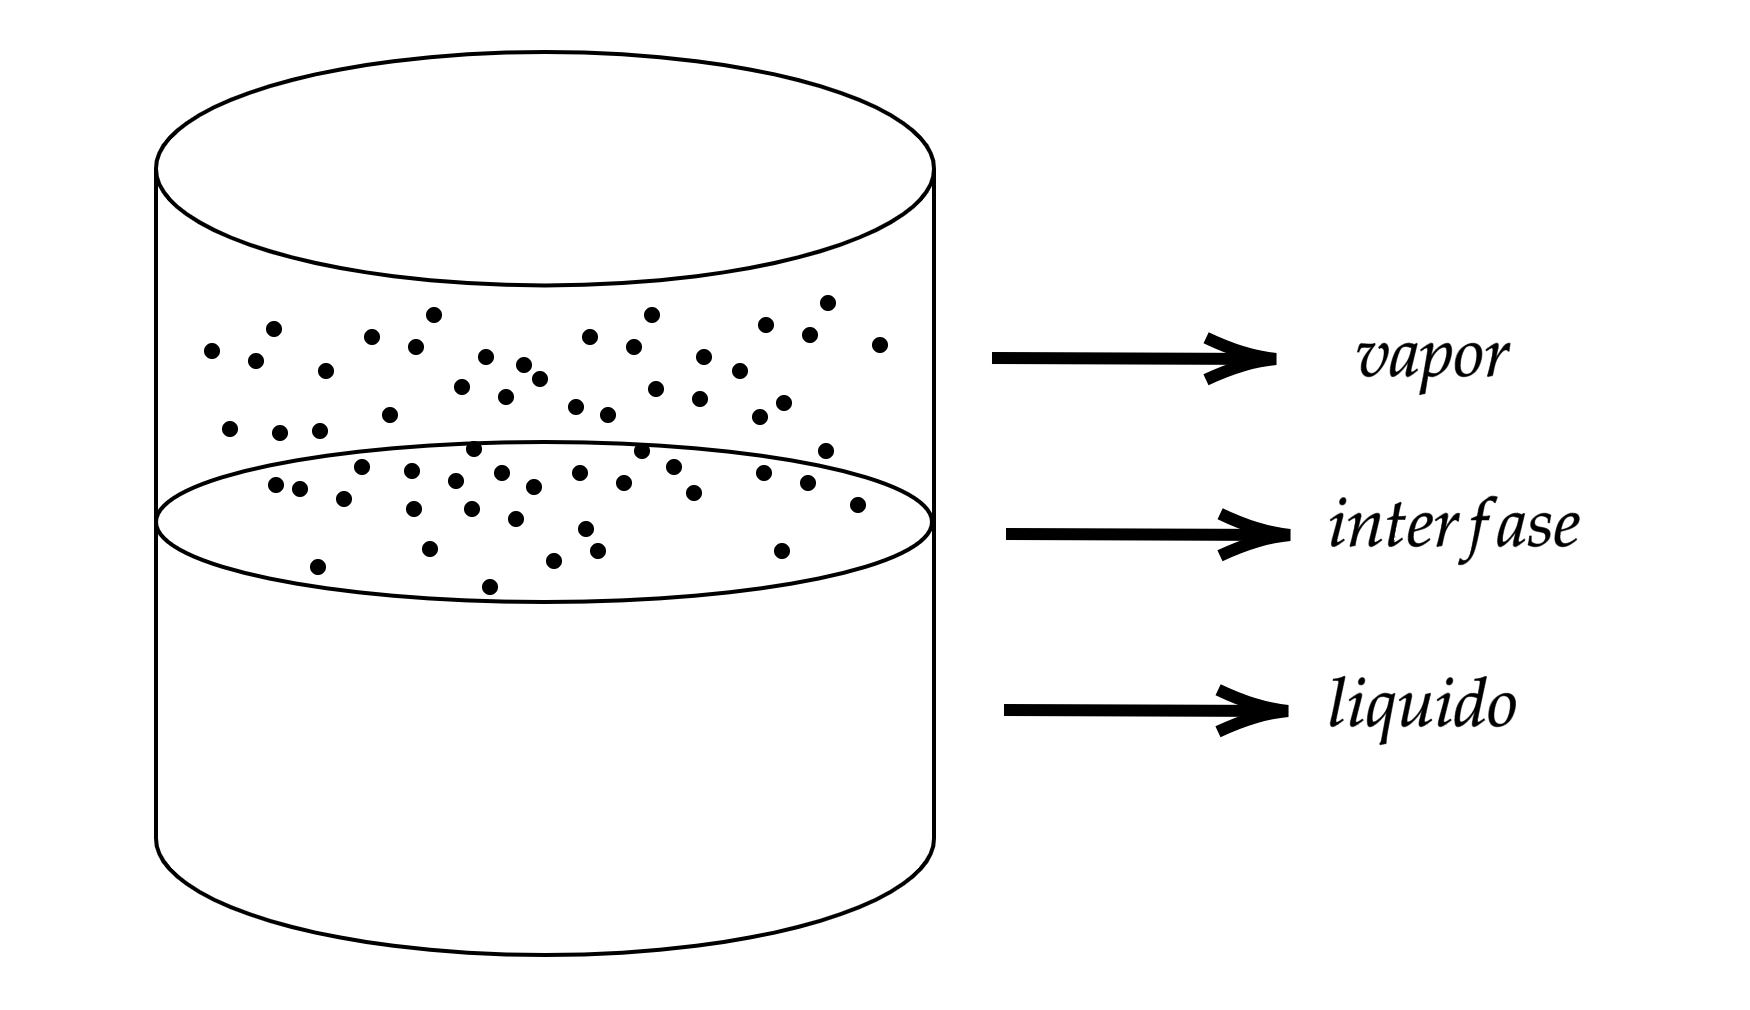
\includegraphics[scale=0.16]{../images/diagram-20221024.png}
    \end{center}
\end{minipage}
\begin{minipage}{0.49\textwidth}
    Se tiene un sistema formado por dos subsistemas cerrados y aislados que se encuentran en fase liquida y la otra en forma de vapor. \\[0.2cm]
    \textbf{¿Que ocurre en la interfase?}
\end{minipage}
\\[0.2cm]
Hallamos la entropía del sistema:
\begin{equation}
    S=S_{\ell}+S_v=cte
\end{equation}
Si lo diferenciamos, obtenemos:
\begin{equation}
    dS=d(S_{\ell}+S_v)=dS_{\ell}+dS_v=0
\end{equation}
Se observa que los "dos subsistemas" tienen que cumplir la Ecuación fundamental de la termodinámica para un sistema abierto monocomponente:
\begin{align}
    TdS=dU+pdV-\mu dN \\
    dS=\dfrac{dU+pdV-\mu dN}{T}
\end{align}
\begin{itemize}
    \item Para la fase liquida:
          \begin{equation}
              dS_{\ell}=\dfrac{dU_{\ell}+p_{\ell}dV_{\ell}-\mu_{\ell} dN_{\ell}}{T_{\ell}}
          \end{equation}
    \item Para la fase de vapor:
          \begin{equation}
              dS_{v}=\dfrac{dU_{v}+p_{v} dV_{v}-\mu_{v} dN_{v}}{T_{v}}
          \end{equation}
\end{itemize}
Reemplazamos en:
\begin{align}
    dS_{\ell}+dS_v=0 \\
    \dfrac{dU_{\ell}+p_{\ell}dV_{\ell}-\mu_{\ell} dN_{\ell}}{T_{\ell}}+\dfrac{dU_{v}+p_{v} dV_{v}-\mu_{v} dN_{v}}{T_{v}}=0
\end{align}
\section{Condiciones del sistema}
\begin{itemize}
    \item \textbf{Energía interna del sistema} \\[0.3cm]
          Si notamos que la energía interna del sistema cumple la siguiente relación:
          \begin{equation}
              U=U_{\ell}+U_v=cte
          \end{equation}
          Si diferenciamos esta relación, obtenemos:
          \begin{align}
              dU_{\ell}+dU_v & =0          \\
              dU_v           & =-dU_{\ell}
          \end{align}
    \item \textbf{Volumen del sistema}\\[0.3cm]
          El volumen del sistema cumple la siguiente relación:
          \begin{equation}
              V=V_{\ell}+V_v=cte
          \end{equation}
          Si diferenciamos esta relación, obtenemos:
          \begin{align}
              dV_{\ell}+dV_v=0 \\
              dV_v=-dV_{\ell}
          \end{align}
    \item \textbf{Numero de componentes del sistema} \\[0.3cm]
          El numero de componentes total del sistema cumple la siguiente relación:
          \begin{equation}
              N=N_{\ell}+N_v=cte
          \end{equation}
          Si diferenciamos esta relación, obtenemos:
          \begin{align}
              dN_{\ell}+dN_v & =0          \\
              dN_v           & =-dN_{\ell}
          \end{align}
\end{itemize}
Reemplazando obtenemos:
\begin{align}
    \left( \dfrac{dU_{\ell}}{T_{\ell}}+ \dfrac{dU_{\ell}}{T_v} \right)+\left( \dfrac{p_{\ell}dV_{\ell}}{T_{\ell}}+\dfrac{p_v dV_{\ell}}{T_v} \right)-\left( \dfrac{\mu_{\ell} dN_{\ell}}{T_{\ell}}-\dfrac{\mu_v dN_{\ell}}{T_v} \right)=0 \\
    \left[ \dfrac{1}{T_{\ell}}-\dfrac{1}{T_v} \right]dU_{\ell}+\left[ \dfrac{p_{\ell}}{T_{\ell}}-\dfrac{p_v}{T_v} \right]dV_{\ell}-\left[ \dfrac{\mu_{\ell}}{T_{\ell}}-\dfrac{\mu_v}{T_v} \right]dN_{\ell}=0
\end{align}
Se observa que $dU_{\ell} \neq 0$, $dV_{\ell} \neq 0$ y $dN_{\ell} \neq 0$. De modo que los términos entre paréntesis se igualan a cero:
\section{Condiciones de equilibrio}
\begin{itemize}
    \item[a)] \textbf{Condición de equilibrio térmico}
        \begin{align}
            \left[ \dfrac{1}{T_{\ell}}-\dfrac{1}{T_v} \right]=0 \\
            T_{\ell}=T_v
        \end{align}
    \item[b)] \textbf{Condición de equilibrio mecánico}
        \begin{align}
            \left[ \dfrac{p_{\ell}}{T_{\ell}}-\dfrac{p_v}{T_v} \right] & =0   \\
            p_{\ell}                                                   & =p_v
        \end{align}
    \item[c)] \textbf{Condición de equilibrio químico}
        \begin{align}
            \left[ \dfrac{\mu_{\ell}}{T_{\ell}}-\dfrac{\mu_v}{T_v} \right]=0 \\
            \mu_{\ell}=\mu_v
        \end{align}
\end{itemize}
\end{document}